\twocolumn[
\begin{center}
\title{\color[cmyk]{1, 0.57, 0, 0.38}{\Huge\bfseries Il nuovo FedoraOnLine: motivazioni e curiosità\\}} % definisco il titolo dell'articolo
\author{\scriptsize Gabriele Trombini (mailga@fedoraonline.it)} % definisco l'autore e altre informazioni
\date{}
\end{center}
{\color[cmyk]{1, 0.46, 0, 0}\LARGE FOL 2 - il percorso pieno di imprevisti}\\
\maketitle
\normalsize
\doublespacing
\hfill
]
\onehalfspacing
\lettrine[lines=1, loversize=0.1, lraise=0.1]{\color[cmyk]{0.5, 0, 1, 0}\bfseries I}{}l nostro webmaster, come molti di voi certamente sapranno, è uno stakanovista del lavoro in FedoraOnLine, un vulcano di idee, ed è sempre pronto a valutare qualsiasi possibilità di crescita.\\

Da molto tempo, all'interno dello staff, si discuteva circa un possibile rinnovamento grafico e concettuale del sito. Le idee erano molte ma la focalizzazione degli strumenti atti a raggiungere lo scopo erano ben remoti dall'essere stabiliti.\\

La questione non si poneva solo in termini di layout, la rivisitazione avrebbe dovuto riguardare la totalità del sito: si trattava di scegliere il cms in sostituzione di Xoops, che ci avrebbe permesso di gestire in maniera più efficace le sezioni presenti.\\

Prese così forma l'obiettivo da raggiungere, che comprendeva sia il cms che dei gestori di contenuti (in primis il forum stesso e la sezione documentazione).\\

Il lavoro che si presentava era decisamente superiore alle forze presenti nello staff, anche perchè il forum ``vecchia versione'' doveva avere continuità.\\

Pertanto, definite le zone di interesse e gli strumenti per la loro gestione (Drupal a livello di cms, fluxbb a livello di forum e mediawiki per la parte documentale), abbiamo cominciato a lavorare sulle varie sezioni, ricercando anche dei validi collaboratori per ottenere i risultati sotto gli occhi di tutti.\\

Virus, Trpost ed io avremmo continuato a gestire il forum insieme, mentre Robyduck, MarioS e Pagnolo avrebbero cominciato a vedere come mettere insieme tutti gli strumenti che erano stati scelti.\\

Era l'estate dell'anno scorso e Virus ci mise a disposizione un server git per poter mettere insieme il lavoro fatto in comune.\\

\begin{figure}[htbp]
\centering
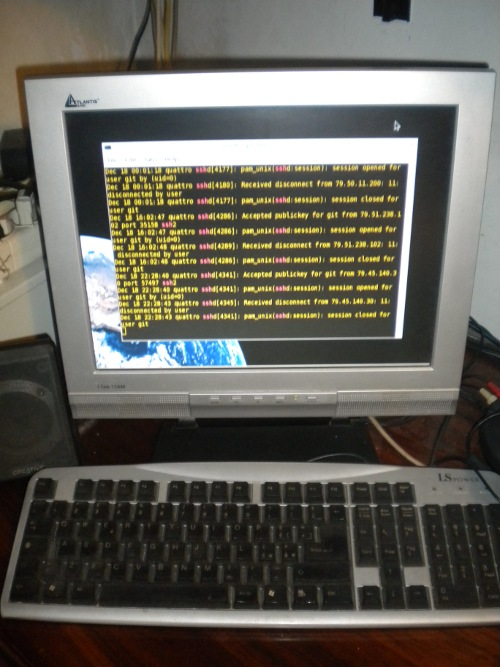
\includegraphics[scale=.10]{articoli/editoriale/immagini/server_git.jpg}
\caption{Il nostro server git\label{Fig.1: server git}}
\end{figure}

Il primo grosso problema che si presentò era il trasferimento del database di Fol versione 1.0 in quello che sarebbe divenuto Fol 2.0, perchè non aveva senso perdere la nostra storia.\\

Il secondo grosso problema, che ci era sembrato insormontabile, inizialmente, era dato dal login unificato tra Drupal e Fluxbb (non aveva senso mantenerlo anche per Mediawiki, visto che solo i redattori iscritti in mailing list, possono fornire contributi).\\

In entrambi i casi il lavoro fu abbastanza duro e richiedemmo aiuto anche ai nostri cugini d'oltralpe di fedora-fr.org, i quali ci indirizzarono verso una soluzione con delle criticità troppo onerose per le nostre energie.\\

Nel frattempo Robyduck e Pagnolo si occupavano della sistemazione grafica, uniformandola nei diversi programmi coadiuvati dai collaboratori per la parte grafica, lo storico Tuzzer ed Ilnanny mentre il nostro MarioS ricercava un modo più semplice per poter fare il login unificato e per il trasferimento dei dati da un database all'altro.\\

Tutto procedeva, a Folio era stata data una priorità ovviamente secondaria, senonchè, a causa di scelte personali Trpost si distaccò dal nostro gruppo di lavoro e impegni lavorativi portavano lontano dal progetto anche Tuzzer.\\

Se contiamo il fatto che alcuni utenti, solitamente presenti e attivi in seno alle notizie ed al forum, che ci avevano dato disponibilità a prendere in mano un settore di interesse, a causa di problemi personali non hanno potuto anch'essi proseguire nella collaborazione, ci siamo trovati, ad un certo punto, in grossa difficoltà.\\

Riassumendo, eravamo bloccati sulla soluzione del login (il trasferimenti da un database all'altro non era più un problema), la gestione del forum aveva subito una defezione, il supporto grafico era dimezzato e alcuni collaboratori non potevano darci una mano.\\

Per di più bisognava cominciare a tracciare le linee per la redazione di Folio.\\

Il tutto faceva prendere una brutta piega al lavoro, che subiva, quindi, un rallentamento.\\

La svolta ci fu quando MarioS ha trovato il modo per il login unico (ricordiamo l'importanza di avere un login nella home del sito e non doverlo ripetere qualora si entri nel forum) e con il mio spostamento sull'attività di Mediawiki (insieme a Robyduck, che si occupava di tutto, e di Zamingas).\\

Mediawiki aveva bisogno di essere impostato per quanto riguarda le due pagine di fondamentale importanza, ``contribuisci'' e ``convenzioni di scrittura'', che furono fatte in breve tempo da me e da Robyduck, dopo aver stabilito che anzichè appoggiarci al server git, per la parte documentale sarebbe stato meglio creare online la sezione.\\

Passammo poi, con il contributo di ilnanny, MarioS stesso e Zamingas, a importare le guide dal vecchio sito al nuovo; operazione tediosa ma relativamente breve.\\

Facendo le somme, a quel punto capimmo che era cominciata la fase di discesa; Drupal era ad un passo dalle rifiniture finali, il forum era stato importato nel nuovo database di Fluxbb, Mediawiki era finito e lo script di login era praticamente terminato.\\

Ormai ce l'avevamo fatta, per cui mi sono buttato a capofitto su Folio, se non che, la mia decisione iniziale di redigerlo con Scribus faceva a pugni con quello che nel web viene solitamente fatto: cioè l'utilizzo di Latex.\\

Dovevo cominciare daccapo, leggere e studiare, studiare e capire un linguaggio non propriamente facile anche se redditizio in termini di resa.\\

A questo punto, ed è storia di oggi, siamo online, con dei ritorni positivi e con l'uscita di questo numero di Folio.\\

\begin{figure}[htbp]
\centering
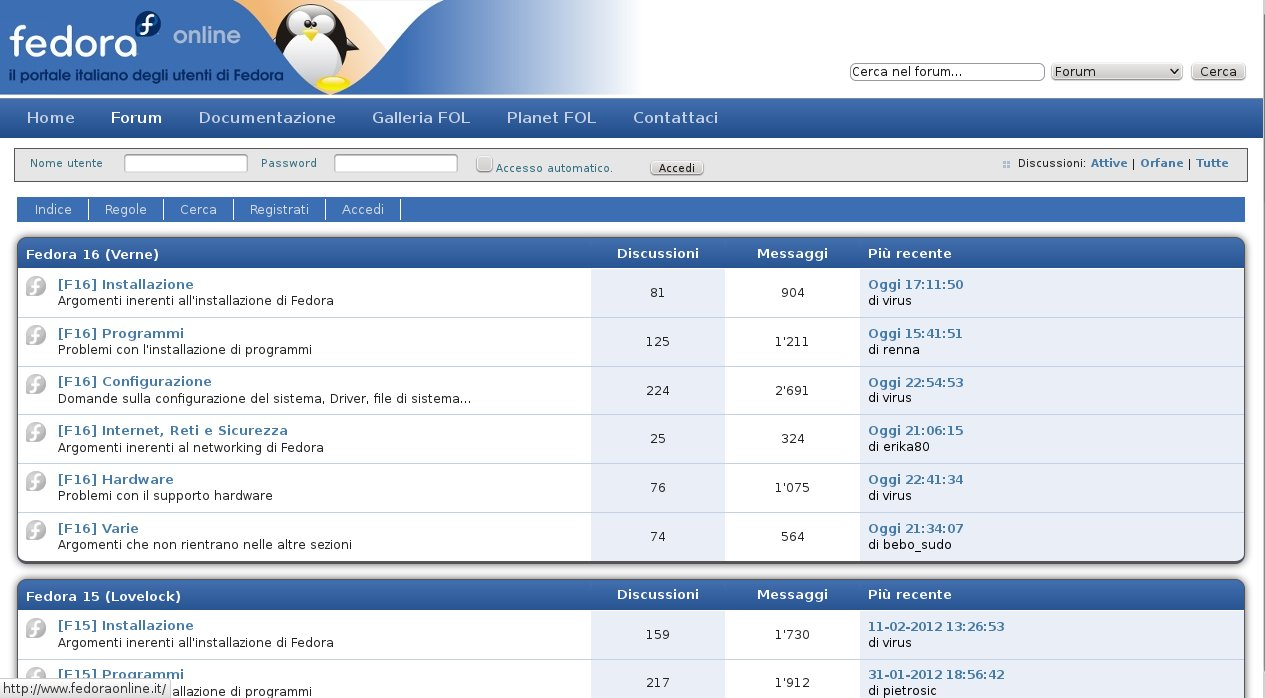
\includegraphics[scale=.20]{articoli/editoriale/immagini/forum_fol.jpeg}
\caption{Il nostro forum\label{Fig.1: forum}}
\end{figure}

La missione è compiuta, siamo orgogliosi di aver messo a disposizione delgli utenti uno strumento che possa dare risposta alle richieste.\\

E Virus?
Ragazzi! Senza Virus che ha retto sulle proprie spalle il carico del forum senza creare disagio agli utenti, non ho difficoltà ad ammettere che probabilmente tutto questo non avrebbe potuto essere così.\\

That's all, folks!

